\section{Problems}
\label{section:problems}

\begin{enumerate}
\def\labelenumi{\arabic{enumi}.}
\item
  Consider a random variable that obeys a uniform density and varies
  from 2 to 5. (a) Determine the mean and variance of the random
  variable. (b) What is the probability that the random variable is
  between 2 and 3? (c) Plot the CDF.
\item
  In Figure 8.7 it was assumed that the CDF function is monotonically
  increasing. That is, \includegraphics{Fig/media/image162.wmf}. Show
  why this is so using equation (13).
\item
  Describe what is meant by \emph{failure rate}, \emph{failure
  function}, and \emph{reliability}.
\item
  Consider an integrated circuit that has
  \includegraphics{Fig/media/image163.wmf}. (a) Determine the mean time
  to failure. (b) Determine the reliability in 5, 10, 15, and 20 years.
\item
  Consider a CD4001BC 2-Input Quad NOR gate (datasheet available in
  Appendix D). Also assume it is a glass-sealed dual inline package, 15
  years in production, \includegraphics{Fig/media/image164.wmf}, the
  power dissipated in the application averages 10mW, it has B-1 quality,
  and that it is to be operated in laboratory equipment at an ambient
  temperature of 25°C. Use the MIL-HDBK-217F data in Appendix C to
  determine the MTTF and estimate its reliability in 25 years.
\item
  Use the MIL-HDBK-217F data in Appendix C to estimate the reliability
  of a 32 bit CMOS microprocessor. Assume that it is used in a missile
  launcher, the ambient temperature is 120°C, that it has 64 pins, that
  it has been in production for 6 months, B-1 quality parts are used,
  and it is a non-hermetic DIP. Determine the MTTF and reliability for
  the microprocessor in 20 years. (Note: this is the same operating
  environment used for the BJT in Example 8.5.)
\item
  Consider a 1N4001 diode (datasheet in Appendix D) that is to be
  operated in the switching circuit shown below. Also assume that the
  part quality is Lower, it is metallurgically bonded, and that it is to
  be used in an airborne inhabited cargo environment at an ambient
  temperature of 50°C. Use the MIL-HDBK-217F data in Appendix C to
  determine the MTTF and estimate its reliability in 25 years.
\end{enumerate}

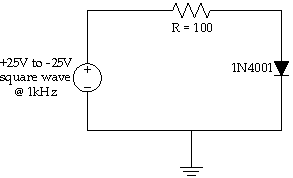
\includegraphics[width=2.5in,height=1.51042in]{Fig/media/image165.emf}

\begin{enumerate}
\def\labelenumi{\arabic{enumi}.}
\setcounter{enumi}{7}
\item
  Use the MIL-HDBK-217F data in Appendix C to determine the reliability
  of the inverting op amp circuit, shown below, in 15 years. Assume that
  it is used in an automotive application (environmental factor =
  G\textsubscript{M}), the ambient operating temperature is
  80\textsuperscript{O}C, industrial quality parts are employed, and ¼
  watt fixed composition resistors of the lowest quality are used. The
  datasheet for the LM741 op amp is in Appendix D. The LM741 is
  considered to be a linear microcircuit, comes in a dual inline package
  (DIP), contains 25 bipolar transistors, has S quality, and has been in
  production for well over 20 years.
\end{enumerate}

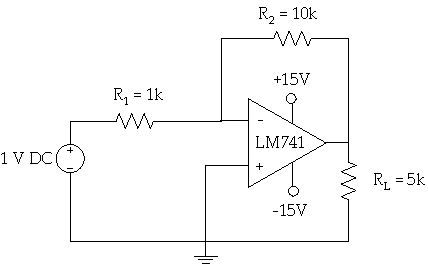
\includegraphics[width=2.8125in,height=1.77083in]{Fig/media/image166.emf}

\begin{enumerate}
\def\labelenumi{\arabic{enumi}.}
\setcounter{enumi}{8}
\item
  Consider the circuit in Example 8.4. Assume that a heat sink is
  attached to the 2N3904 BJT (datasheet in Appendix D) and it has the
  following thermal resistance values
  \includegraphics{Fig/media/image167.wmf} and
  \includegraphics{Fig/media/image168.wmf}. If the device is operated at
  an ambient temperature of 130°C, determine the maximum power
  dissipation of the BJT and its reliability in 50 years.
\item
  Your company intends to design, manufacture, and market a new RAID
  (Redundant Array of Independent Disks) for network servers. The system
  must be able to store a total of 500GB of user data and must have a
  reliability of at least 95\% in 10 years. In order to develop the RAID
  system, 20GB drives will be designed and utilized. To meet the
  requirement, you have decided to use a bank of 25 disks
  (25x20GB=500GB) and utilize a system redundancy of 4 (each of the 25
  disks has a redundancy of 4). What must the reliability of the 20GB
  drive be in 10 years in order to meet the overall system reliability
  requirement?
\item
  \includegraphics{Fig/media/image106.wmf} has a failure probability of
  2\% and \includegraphics{Fig/media/image169.wmf} has a failure
  probability of 3\%. \includegraphics{Fig/media/image170.wmf},
  \includegraphics{Fig/media/image171.wmf},
  \includegraphics{Fig/media/image172.wmf}, and
  \includegraphics{Fig/media/image173.wmf} are identical redundant
  systems. Determine the required reliability of the redundant systems
  necessary for the overall system to have a reliability of 94\%.
\end{enumerate}

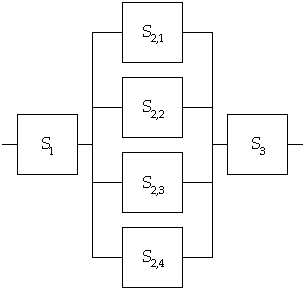
\includegraphics[width=2.0625in,height=1.96875in]{Fig/media/image174.emf}

\begin{enumerate}
\def\labelenumi{\arabic{enumi}.}
\setcounter{enumi}{11}
\item
  Consider the design of a triply-redundant majority voting system, with
  three binary inputs a, b, and c shown below. The inputs represent data
  from 3 independent sources from which the objective is to determine if
  the majority of the input bit values are logic level 0 or 1. Each
  majority circuit outputs the bit value that is in the majority of the
  inputs. The output of each majority circuit is fed into a resistor and
  LED (light emitting diode) network. The LEDs are lit if the output of
  the majority circuit is a logic 1, otherwise the LED is off. Ideally,
  all three LEDs are lit if the majority of inputs is 1, else they are
  all off. However, if part of the system fails, the LED readings may
  not be reliable, so a majority rules decision is used on the LEDs. The
  criterion used is that if two or more LEDs are on, then the majority
  of inputs are considered to be high, otherwise, the majority of inputs
  are considered to be low. Determine the probability of a false reading
  based upon this criterion if each component in the system (gate,
  resistor, or LED) has a reliability of 90\%.
\end{enumerate}

\begin{quote}
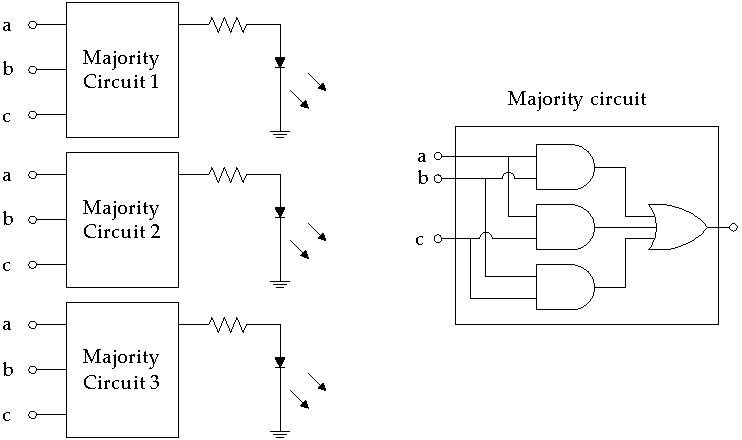
\includegraphics[width=4.1875in,height=2.48958in]{Fig/media/image175.emf}
\end{quote}
